\documentclass[11pt,a4paper]{article}

\usepackage{amsmath,amssymb}
\usepackage{graphicx}
\usepackage{epsfig}
\usepackage{dirtytalk}

\begin{document}

\title{IMRaD style}
\author{Hans Krister Frisk}
\maketitle

\begin{abstract}
 An abstract should give a short and interesting description
 of the contents of the document. You can add a table of contents to your document, by using the command
\say{tableofcontents}. Insert this command in your code, right after the abstract.
\end{abstract}

\tableofcontents

\section{Introduction}

  When you use \LaTeX~there is no risk that a heading ends up at
  the bottom of a page and the text on the following one. Also
  observe that the first paragraph of a chapter or a section is
  never indented. If you type two or more spaces after one
  another like this:                       it will only be
  regarded as one.
	
	A new paragraph is indicated by an empty row in the code and by
  a new row with indentation in the typesetted document. Two or
  more empty rows after one another will be regarded as one. As
  you can see, the first row of this paragraph is indented.
  The
  final
  result
  does
  not
  depend
  on
  where
  you
  insert
  new
  lines
  in
  the
  code.
  % This sentence will not be included in the document.
	
	In the quotation below I show how to do make references. See the list at the end of the paper.
	\say{The connections between number theory and physics have been much studied in
recent years \cite{numb1}. Two main directions in the research are zeta
function techniques and p-adic numbers in high energy physics \cite{numb2}
and the Riemann zeta function as a source of inspiration in low-energy
quantum chaos \cite{qc1}.}
	
	\subsection{An intermediate heading}

  A new section. Notice that \LaTeX\ controls how headings are
  enumerated. Usually all enumerated headings will show up
  automatically in the table of contents. Usually subsections are longer than this one.

  \subsubsection{A subheading}

  The body text is typesetted with a straight right margin, and
  since the hyphenation works well in \LaTeX, there will be no
  large gaps between the words on a row.

  \subsubsection{Yet another subheading}

  Footnotes should only be used in exceptional cases, even if
  they are easy to include.\footnote{This is a footnote.}

  \subsection{Next intermediate heading}

  Here we have moved up one level in the heading hierarchy.
  Notice that the heading is enumerated correctly by \LaTeX.

  \subsubsection{The third subheading}

  If you want to emphasize something, like a word or a phrase,
  you could write it in \emph{italics} or \textbf{boldface}.
  Other available fonts are \textsl{slanted}, \textsc{small
  caps}, \textsf{sans serif}, and \texttt{typewriter}. It is
  also possible to modify the size of the text:
  \begin{center}
    {\Large This} sentence {\LARGE looks}
    {\tiny very} {\large strange}{\Huge !}
  \end{center}
	
	\section*{Headings without numbers}

  If you wish to suppress the enumeration of a section, you
  add an asterisk directly after the section command. This
  also works for intermediate headings and subheadings.
  Headings without a number will not show up in the table of
  contents.

  \section{More examples}

  We continue this overview by looking at more editorial
  structures and how one includes them in a \LaTeX\ document.
	
	
  \subsection{Lists}

  A simple bulleted list:
  \begin{itemize}
  \item First item
  \item Second item
  \item Third item
  \end{itemize}
	
	An enumerated list with three sublists:
  \begin{enumerate}
  \item First item
  \item The second item contains a sublist
    \begin{enumerate}
    \item The first item of the sublist contains in turn yet
      another sublist
      \begin{enumerate}
      \item First item of the subsublist
      \item Second item of the subsublist
      \end{enumerate}
    \item Second item of the sublist
    \end{enumerate}
  \item The third item consists of a longer text that will not
    end until later. Namely after the next sentence. This is
    the last sentence of this item.
  \end{enumerate}
  It is possible to nest lists in at most four levels.
	
	\subsection{Formulae}

  A mathematical equation within a paragraph must be put
  between two dollar signs. An interesting equality is
  $e^{i\pi} + 1 = 0$. Any formula is read from the left to the
  right. The previous formula reads ``e raised to i pi, plus
  one, equals zero''.
	A few examples more: $f_n = f_{n - 1} + f_{n - 2}$ and
  $a^{(p - 1)/2} \equiv 1 \pmod{p}$.


  Equations, that are important or take too much space within
  a paragraph, should be displayed. Often you wish to refer to
  a equation later (or earlier) in the text. We can tell
  \LaTeX\ to number such an equation in the right margin:
  \begin{equation}
    \label{eq:summa}
    1 + 2 + 3 + \dots + n = \frac{n(n + 1)}{2}.
  \end{equation}
  The equation~\eqref{eq:summa} is well-known to mathematicians
  and is applied every now and then. If you don't want any number
	of the equation you write the command \say{nonumber} to the right in the equation.
	Don't forget the backslash in front of it.
	Here comes yet another displayed equation, but this one has
  no number assigned to it:
  \[
    \frac{\sin m x}{\sin x}
    = (-4)^{(m - 1)/2} \prod_{j = 1}^{(m - 1)/2}
    \left(\sin^2 x - \sin^2 \frac{2 \pi j}{m}\right).
  \]
	
	 It is even possible to make tables. The following table was valid as of August 23rd, 2012.
  \begin{center}
    \begin{tabular}{lllr}
      \hline
      \textbf{Name}  & \textbf{Country} &
      \textbf{Event} & \textbf{Result}  \\
      \hline
      Therese Alshammar & Sweden         & 50 m butterfly
        &   25.07 \\
      David Rudisha     & Kenya          & 800 m
        & 1:40.91 \\
      Jan \u{Z}elezn\'y & Czech Republic & Javelin
        &   98.48 \\
      Sergey Bubka      & Ukraine        & Pole vault
        &    6.14 \\
      \hline
    \end{tabular}
  \end{center}

\section{Results}

I use eps format for plots but you can use pdf also but then you have to
use another package.
Important that eps-file lies in same folder as this tex-document.
\begin{figure}[tbph]
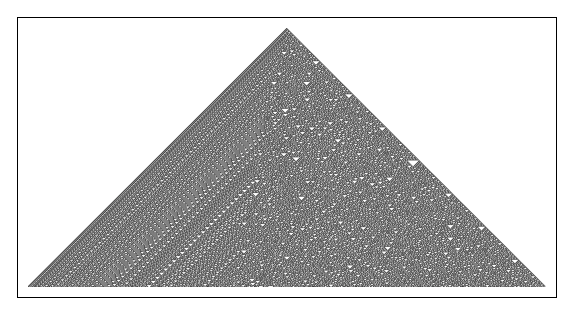
\epsfig{file=plot1.eps}
\caption{ This figure illustrates three geometrical concepts.
Point, circle and line. It is done with Graphics command in Mathematica.}
\end{figure}

There it came! Now we have a look at the second figure. Unfortunately it will not appear exactly where
you want it to be.
\begin{figure}[tbph]
\epsfig{file=plot4.eps}
\caption{ The curve is $\sin x$ and the line $\frac{x}{2}$. To solve
the equation $\sin x = \frac{x}{2}$ a numerical method is needed. 
}
\end{figure}
 To get it on paper you use Build, or Build and View, in TeXnicCenter. If you have eps-files
use LaTeX $\rightarrow$ PS $\rightarrow$ PDF in the box.  LaTeX $\rightarrow$ PDF also works fine. Figure 2 came out below this text.
Disturbed by Out sign to the very left in the plot? You can cut them in Mathematica. Do you want frame, axes labels etc
for your plot? No problem, see Plot command in Mathematica. You write Plot, mark it with mouse and select
Find Selected Function in the help menu.

\section{Discussion}
You end with a discussion and conclusions. When you compile your tex-file do it TWICE to get references etc right.

\begin{thebibliography}{99}
\bibitem{numb1}  L. Brekke and P. G. O. Freund, Phys. Rep. 233 (1993) 1-66;
E. Elizalde, "Ten Physical Applications of Spectral Zeta Functions", Springer
-Verlag, 1995.

\bibitem{numb2}  V. S. Vladimirov, I. V. Volovich and E. I. Zelenov,
''P-adic Analysis and Mathematical Physics'', World Scientific, 1995;


\bibitem{qc1}  M.Berry and J. Keating, Siam Review 41, (1999), 236-266.
\end{thebibliography}

\end{document}
